\chapter{Data Preprocessing}

In this section, we describe the data preprocessing steps performed on the merged dataset. The preprocessing phase is crucial in preparing the data for further analysis by cleaning it and transforming it into a suitable format for modeling. This is done in Python using the Pandas library. 

\section{Dataset Overview}

We start by loading and exploring the dataset using the following commands:

\begin{verbatim}
# Display the first few rows of the dataset
df.head()

# Display basic information about the dataset
df.info()
\end{verbatim}

\begin{figure}[h]
    \centering
    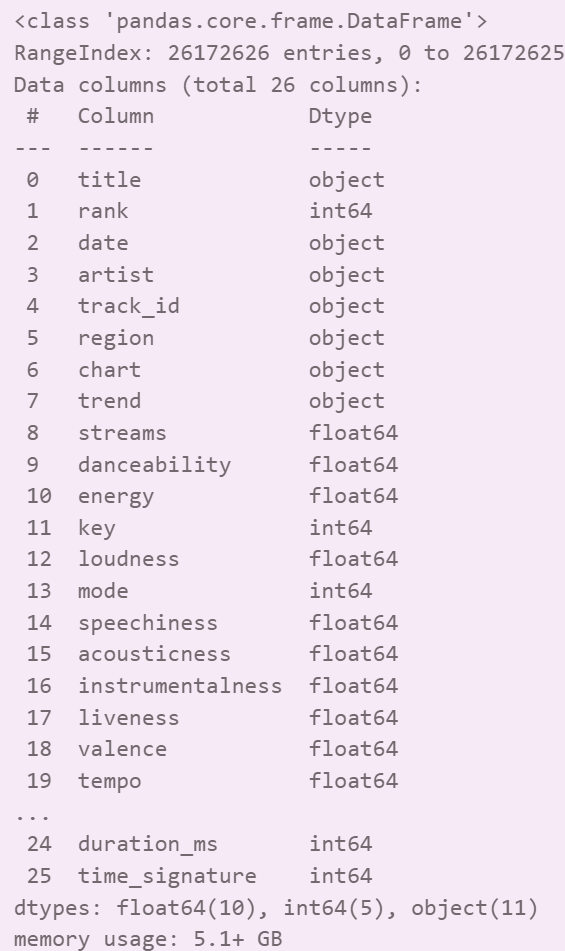
\includegraphics[width=0.5\textwidth]{media/info.png} 
    \caption{Basic information.}
    \label{df.info()}
\end{figure}

\newpage
\begin{verbatim}
# Summary statistics of the dataset
df.describe()
\end{verbatim}


\begin{figure}[h]
    \centering
    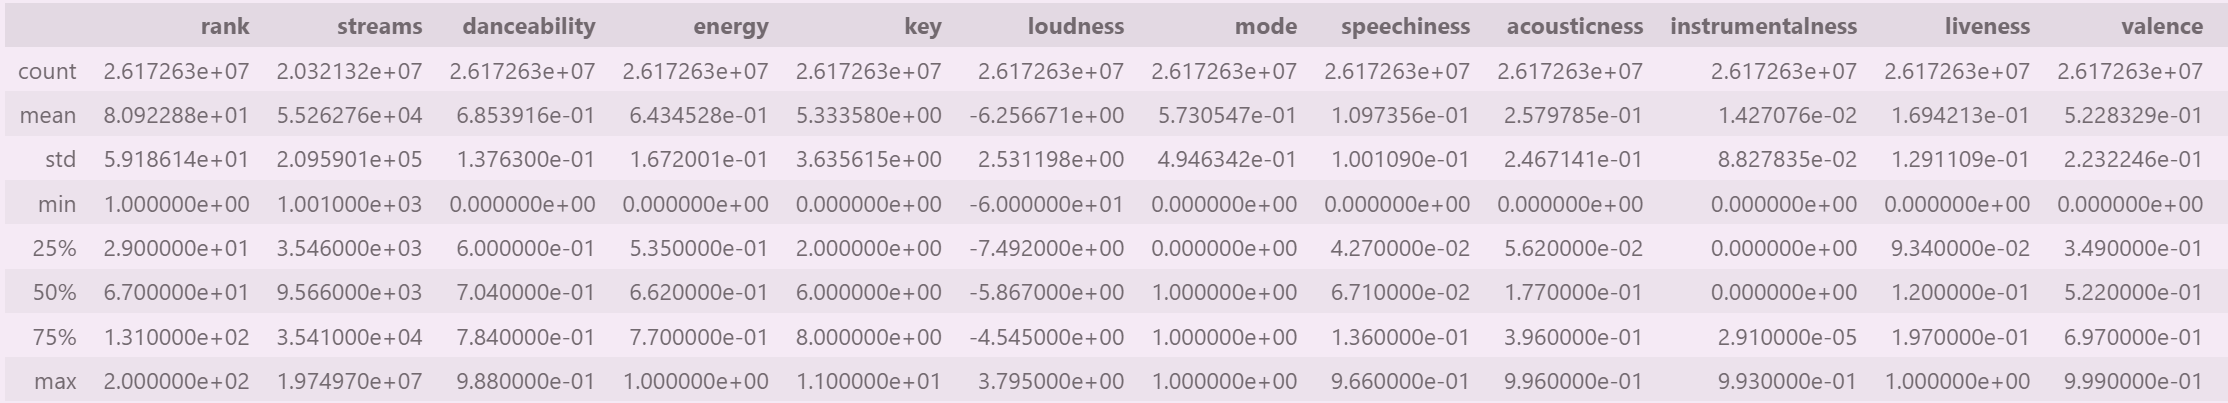
\includegraphics[width=1.1\textwidth]{media/describe.png} 
    \caption{Summary statistics of the dataset.}
    \label{df.describe()}
\end{figure}




\subsection{Missing Values Detection}

We check for missing values in the dataset using the following methods:

\begin{verbatim}
# Check for missing values in each column
df.isna().sum(axis=0)
\end{verbatim}

The columns with missing values are: streams, title and artist. These columns are not useful for the analysis and can be removed.


Other columns such as date, chart, trend, etc... don't contribute to the analysis and can be removed.


After removing these columns, we check again for missing values to ensure a clean dataset and confirm that there are no missing values left.
This allowed us to reduce the number of columns from 25 to 16.



\section{Grouping Regions}

We group countries into 11 geographical regions: Northern Europe, Eastern Europe, Western Europe, Southern Europe, North America, Latin America, East Asia, South Asia, Middle East, Oceania, and Africa. A mapping function is used to assign each country to a group.

\begin{verbatim}
# Mapping of countries to regions
regions_mapping = {
    'Latin America': ['Argentina', 'Bolivia', ...],
    'North America': ['Canada', 'United States'],
    'Northern Europe': ['Denmark', 'Finland', ...],
    ...
}
    
# Update the 'region' 
for region, countries in regions_mapping.items():
    df.loc[df['region'].isin(countries), 'region'] = region
\end{verbatim}




In cases where the same song appears more than once in a region, we calculate the mean rank and add a new column \texttt{frequency} to represent how many times the song appears in the chart.

\begin{verbatim}
# Define the regions you want to check
regions_to_check = ['Latin America', 'Oceania', 'Western Europe', 'Eastern Europe', ...]
    
# Filter the DataFrame to include only rows from the specified regions
df_filtered = df[df['region'].isin(regions_to_check)]
    
# Group by 'track_id' and 'region' to calculate the mean of 'rank' and the frequency (count of occurrences)
df_grouped = df_filtered.groupby(['track_id', 'region']).agg({
    'rank': 'mean',    # Mean of rank 
    'track_id': 'size' # Count of occurrences 
}).rename(columns={'rank': 'rank_mean', 'track_id': 'frequency'}).reset_index()
\end{verbatim}

The chart dataset initially had about 20 million rows. By identifying the unique songs IDs for each region, we managed to decrease to 200K rows.

We visualize the distribution of songs for each regional group.


\begin{figure}[h]
    \centering
    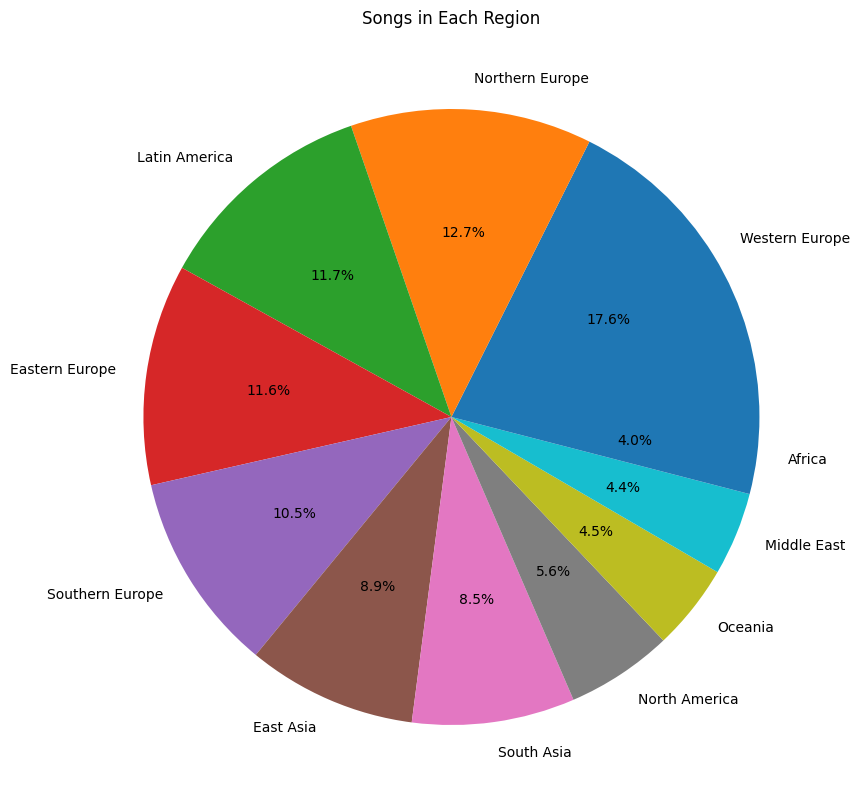
\includegraphics[width=0.7\textwidth]{media/region_songs.png} 
    \caption{Distribution of songs across regions.}
    \label{pie_chart}
\end{figure}


Now the song IDs can be removed since they are not needed for further analysis:

\begin{verbatim}
# Drop the 'track_id' column
df_final = df_final.drop(columns=['track_id'])
\end{verbatim}

\section{Outlier Detection}

We plot box plots for each feature to visualize the distribution and detect outliers. Based on this analysis, we decide whether to remove outliers.

\begin{verbatim}
# List of features
features = ['danceability', 'energy', 'key', 'loudness', 'mode', 'speechiness', 'acousticness', 
'instrumentalness', 'liveness', 'valence', 'tempo', 'duration_ms', 'time_signature']
    
# Create box plots for each feature
plt.figure(figsize=(15, 10))
for i, feature in enumerate(features, 1):
    plt.subplot(4, 4, i)
    sns.boxplot(x=df_final[feature])
    plt.title(f'Box Plot of {feature}')
plt.tight_layout()
plt.show()
\end{verbatim}

\newpage

\begin{figure}[h]
    \centering
    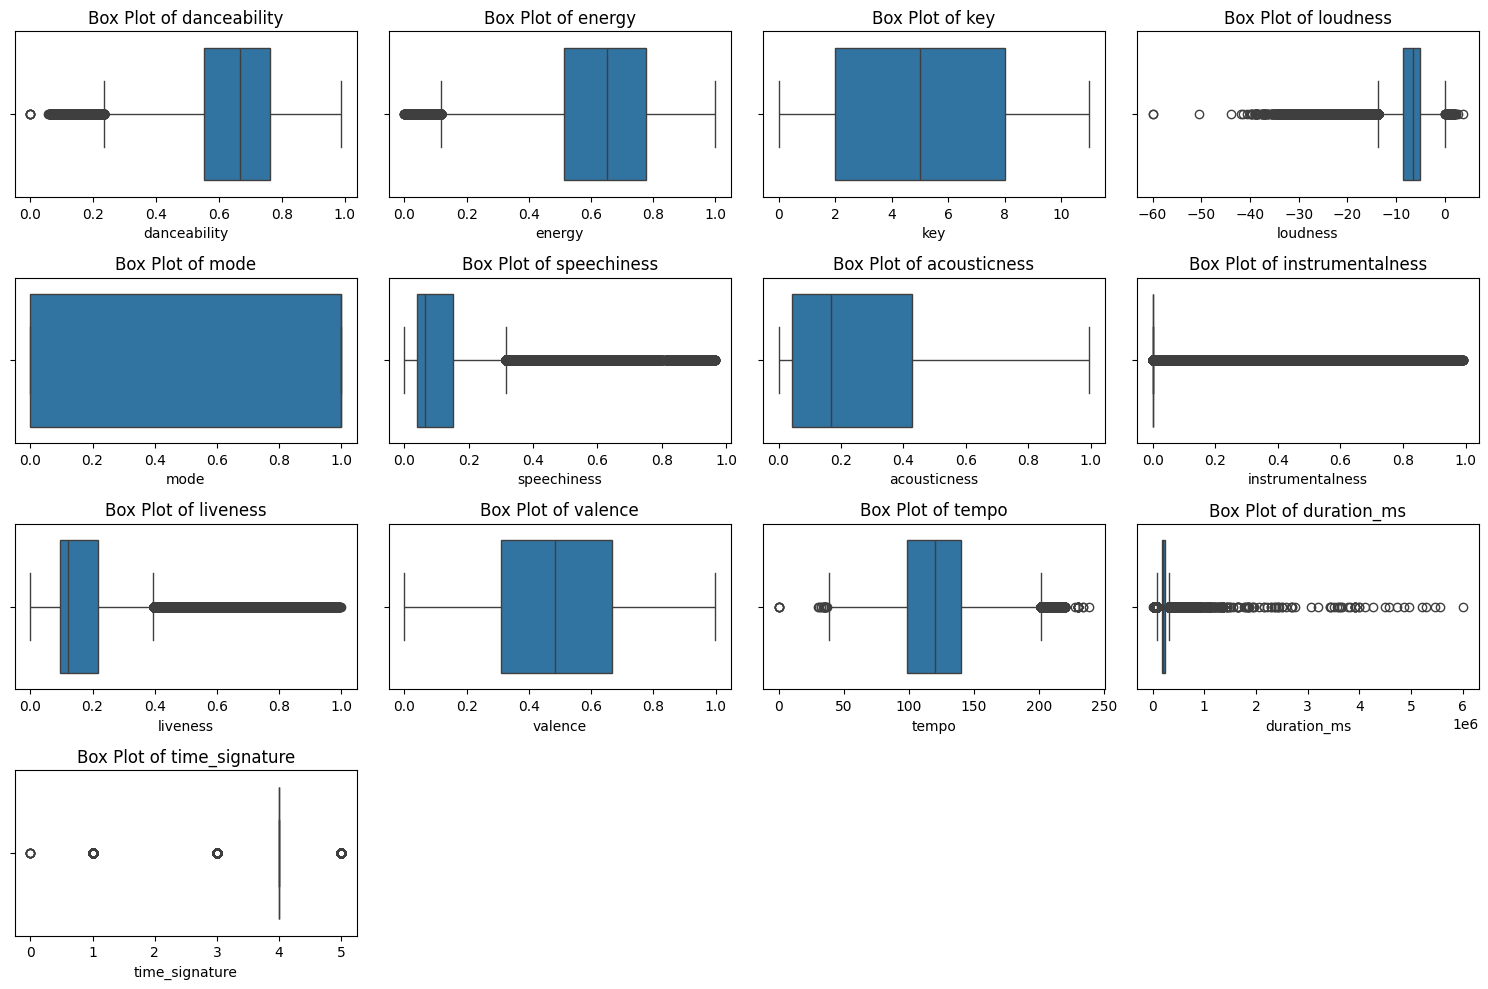
\includegraphics[width=0.8\textwidth]{media/outlier.png} 
    \caption{Box plot of audio features.}
    \label{box_plot}
\end{figure}


The box plots in Figure \ref{box_plot} show the distribution of various features in the dataset and help identify potential outliers.

\begin{itemize}    
    \item \textbf{Loudness}: The loudness feature has numerous outliers on the lower end, extending below -40 dB. This suggests that some tracks in the dataset have exceptionally low loudness levels, possibly due to poor audio quality or artistic choice.

    \item \textbf{Speechiness and Instrumentalness}: Both of these features exhibit a long tail of outliers. Speechiness has many values close to 0, with a few outliers extending towards 1, indicating tracks that are more spoken-word focused. Instrumentalness shows a dense concentration near 0 but also has numerous outliers, possibly representing fully instrumental tracks.

    \item \textbf{Liveness, and Valence}: Liveness shows some outliers, particularly above 0.8, which could represent live recordings. Valence, indicating the musical positivity, shows a broad range without many extreme outliers.

    \item \textbf{Tempo and Duration (in ms)}: Tempo has several outliers at the higher end above 200 BPM, while duration has many high outliers above 4 million milliseconds (about 66 minutes). These extreme values in duration suggest that some tracks are abnormally long, potentially representing extended live performances or podcasts.

    \item \textbf{Time Signature}: This feature contains categorical values, and outliers are represented by infrequent time signatures (e.g., 1, 3, and 5), which are less common in modern music compared to the standard 4/4 time signature.
\end{itemize}


Outliers can potentially distort the analysis and the behavior of models. 

\newpage
To remove outliers in a more secure way, we use the Mahalanobis distance to detect and eliminate extreme values.

\begin{verbatim}
# Subset of the data for the relevant features
data_features = df_final[features]

# Mean and covariance of the features
mean = np.mean(data_features, axis=0)
cov_matrix = np.cov(data_features.values.T)
inv_cov_matrix = np.linalg.inv(cov_matrix)

# Function to compute Mahalanobis distance for each point
def mahalanobis_distance(row, mean, inv_cov_matrix):
    return mahalanobis(row, mean, inv_cov_matrix)

# Apply the function to each row of the dataset
data_features['mahalanobis_dist'] = data_features.apply(lambda row: mahalanobis_distance(row, mean, inv_cov_matrix), axis=1)

# Set threshold using chi-square distribution (95% confidence level)
threshold = chi2.ppf(0.95, df=data_features.shape[1]-1)  # df is the number of features

# Identify outliers (those with Mahalanobis distance greater than the threshold)
data_features['outlier'] = data_features['mahalanobis_dist'] > threshold

\end{verbatim}

The Mahalanobis distance is a useful metric for detecting outliers in multivariate data. By calculating the distance of each data point from the mean in a multidimensional space, we can identify observations that are significantly different from the rest of the dataset. In this case, we use the Mahalanobis distance to detect outliers in the audio features of the songs. The threshold is set based on the chi-square distribution to ensure a 95\% confidence level. The number of outliers is then counted to assess the impact of removing them from the dataset.
We found that the number of outliers is 61, which is a small fraction of the total dataset. These outliers can be removed to improve the quality of the data for further analysis.


We showed the distribution of the rank mean and of the frequency of the songs in the dataset.

\begin{figure}[h]
    \centering
    \begin{subfigure}[b]{0.45\textwidth}
        \centering
        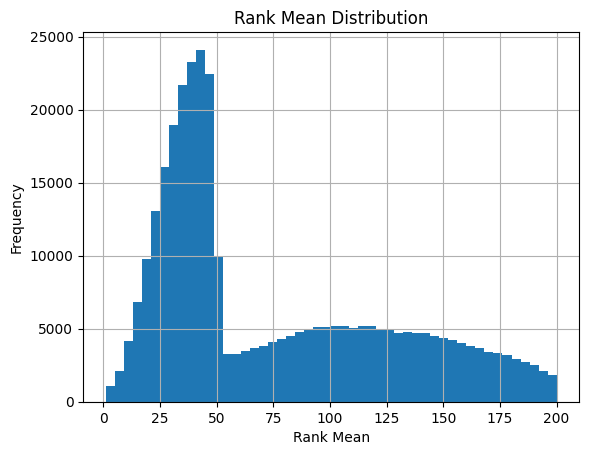
\includegraphics[width=\textwidth]{media/rank_distpng.png}
        \caption{Distribution of the rank mean.}
        \label{rank_mean_distribution}
    \end{subfigure}
    \hfill
    \begin{subfigure}[b]{0.45\textwidth}
        \centering
        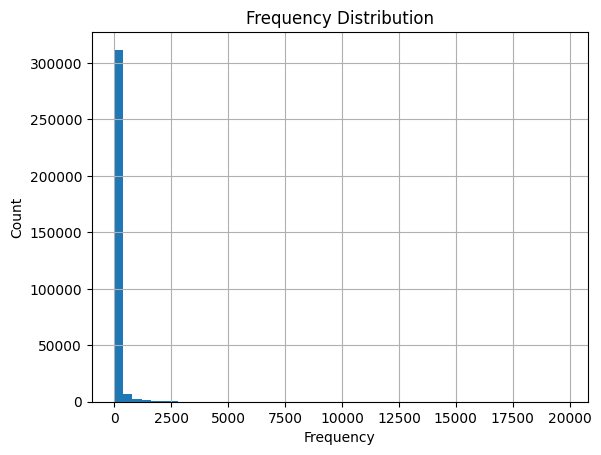
\includegraphics[width=\textwidth]{media/freq_dist.png}
        \caption{Distribution of the frequency of songs.}
        \label{frequency_distribution}
    \end{subfigure}
    \caption{Comparison of the rank mean and frequency distributions.}
    \label{fig:rank_and_frequency}
\end{figure}

Figure \ref{rank_mean_distribution} illustrates the distribution of the rank mean across all songs in the dataset. The rank mean reflects the average position of a song on the charts. Most songs have a rank mean below 50, with a sharp decline after this point. This suggests that a large proportion of songs in the dataset perform well in terms of chart rankings. However, there is a tail of songs with higher rank means, indicating those that appear lower in the charts.

Figure \ref{frequency_distribution} shows the distribution of the frequency of songs in the charts, representing how many times each song appeared in the rankings. The distribution is heavily skewed to the left, with the majority of songs appearing in the charts only a few times. A small number of songs have appeared much more frequently, though this occurrence is rare, as indicated by the long tail of the distribution. This suggests that while most songs have limited presence on the charts, a few songs maintain a significant chart presence over time.



\subsection{Labeling Songs}

We define a threshold to determine whether a song is popular or not. A binary column \texttt{Popular} is added where 0 represents non-popular songs and 1 represents popular songs:

\begin{verbatim}
# Calculate percentiles for rank_mean and frequency
rank_threshold = df['rank_mean'].quantile(0.4)  # 30th percentile
frequency_threshold = df['frequency'].quantile(0.6)  # 75th percentile

# Apply the thresholds
df['popular'] = 0
df.loc[(df['rank_mean'] < rank_threshold) & (df['frequency'] > frequency_threshold), 'popular'] = 1
\end{verbatim}

We discovered that about 80\% of the songs in the dataset are non-popular, while the remaining 20\% are popular.

We can delete the rank\_mean and frequency columns, since they're not needed for further analysis.


\section{Encoding Regional Groups}

We encode the \texttt{Region} column into numerical values:

\begin{verbatim}
df['region']=le.fit_transform(df['region'])
label_mapping = dict(zip(le.classes_, le.transform(le.classes_)))
print(label_mapping)
\end{verbatim}

The regional groups are encoded as follows:
\begin{verbatim}
{'Africa': 0, 'East Asia': 1, 'Eastern Europe': 2, 'Latin America': 3, 'Middle East': 4, 
'North America': 5, 'Northern Europe': 6, 'Oceania': 7, 'South Asia': 8, 
'Southern Europe': 9, 'Western Europe': 10}
\end{verbatim}




The final dataset contains cleaned and transformed features, with only numerical values, ready for analysis. The features include popularity, encoded regional groups and the audio features.

